\documentclass[UTF8]{ctexart}
\usepackage{geometry, CJKutf8}
\geometry{margin=1.5cm, vmargin={0pt,1cm}}
\setlength{\topmargin}{-1cm}
\setlength{\paperheight}{29.7cm}
\setlength{\textheight}{25.3cm}

% useful packages.
\usepackage{amsfonts}
\usepackage{amsmath}
\usepackage{amssymb}
\usepackage{amsthm}
\usepackage{enumerate}
\usepackage{graphicx}
\usepackage{multicol}
\usepackage{fancyhdr}
\usepackage{layout}
\usepackage{listings}
\usepackage{float, caption}

\lstset{
	basicstyle=\ttfamily, basewidth=0.5em
}

% some common command
\newcommand{\dif}{\mathrm{d}}
\newcommand{\avg}[1]{\left\langle #1 \right\rangle}
\newcommand{\difFrac}[2]{\frac{\dif #1}{\dif #2}}
\newcommand{\pdfFrac}[2]{\frac{\partial #1}{\partial #2}}
\newcommand{\OFL}{\mathrm{OFL}}
\newcommand{\UFL}{\mathrm{UFL}}
\newcommand{\fl}{\mathrm{fl}}
\newcommand{\op}{\odot}
\newcommand{\Eabs}{E_{\mathrm{abs}}}
\newcommand{\Erel}{E_{\mathrm{rel}}}

\begin{document}
	
	\pagestyle{fancy}
	\fancyhead{}
	\lhead{王琰博, 3220105837}
	\chead{四则混合运算器}
	\rhead{Dec.16th, 2024}
	
    \section{expression函数的设计思路}
    代码中首先设计了整体的Calculator类,负责封装整个运算流程的相关函数。在之中又嵌套了ExprTree类来实现对中缀表达式的处理,中缀表达式处理操作主要如下:
    
    将表达式拆分成树状结构,根据表达式树的性质,自下往上计算,操作数为叶子节点任意节点的优先级小于等于其子节点的优先级,优先级从高到低依次为:操作数;乘除;加、减。

    所以在对树进行插入操作时,如果表达式树为空则可直接将当前节点作为根节点。如果表达树不为空,则需要考虑优先级与上一节点的关系了。如果优先级更大,则这一节点作为上一个节点的右子节点。如果优先级小,则从上一个节点沿路径向根节点回溯,找到第一个优先级小于当前节点的节点,再将上一个节点作为当前节点的左子节点。

    如果有括号则可以先计算括号内子表达式的结果再将其作为一个数插入树中。

    按照要求本项目也考虑了非法输入的各种情况,通过if的结构对其中可能出现的非法情况进行列举,最终打印ILLEGAL并throw出来。

    另外本运算器还设计了对负数的运算操作,如果当前字符是 - 且它是表达式的第一个字符,或者它的前一个字符是左括号,则认为它是负号而不是减号。最后我们会将负数作为一个完整的字符串进行操作。
	\section{测试程序的设计思路}
	
    测试程序我们考虑了许多情况,首先是对运算结果的计算。随机设计了一些具有括号的较复杂的中缀运算式以及较为简单的运算式作为验证的例子。 
		
    其次我们验证了负数的合法输入以及正确计算结果的功能。

    最后就是设计各种非法输入来检验运算器对非法表达式的识别。

    整体而言表现是好的。设计结果如图所示

    	\begin{figure}[H] %H为当前位置,!htb为忽略美学标准,htbp为浮动图形
			\centering %图片居中
			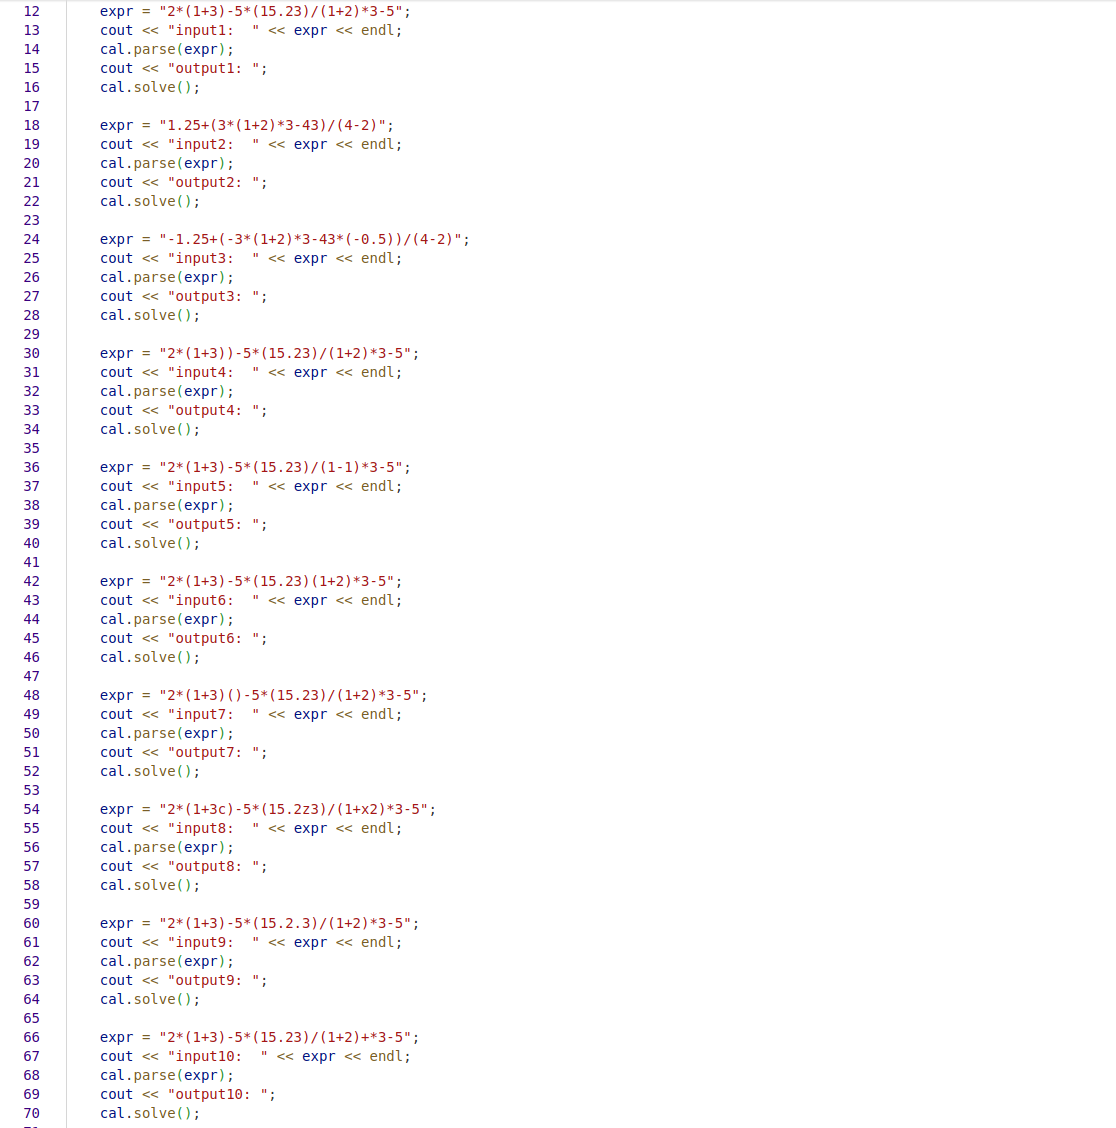
\includegraphics[width=0.7\textwidth]{fig1} %插入图片,[]中设置图片大小,{}中是图片文件名
			\caption{output} %最终文档中希望显示的图片标题
			\label{Fig.test} %用于文内引用的标签
		\end{figure}

	\section{测试的结果}
	
	测试结果如图所示。非法表达式全部输出ILLEGAL,合法表达式全部输出正确结果,我已用计算器进行过验证。
	 
		
		\begin{figure}[H] %H为当前位置,!htb为忽略美学标准,htbp为浮动图形
			\centering %图片居中
			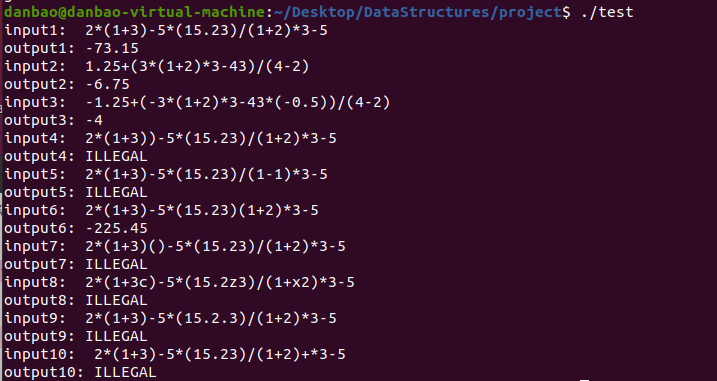
\includegraphics[width=0.7\textwidth]{fig2} %插入图片,[]中设置图片大小,{}中是图片文件名
			\caption{output} %最终文档中希望显示的图片标题
			\label{Fig.output} %用于文内引用的标签
		\end{figure}
		
	
	\section{bug报告}
	
	一切正常。
	
	%%% Local Variables: 
	%%% mode: latex
	%%% TeX-master: t
	%%% End: 
\end{document}